\documentclass[a4paper, 12pt, titlepage]{article}

\usepackage{graphicx, color} %for å inkludere grafikk
\usepackage{verbatim, color} %for å inkludere filer med tegn LaTeX ikke liker. \verbatiminput{verb.txt}
%\usepackage{gensymb} %gensymb Symbols Defined to Work in Both Math and Text Mode 

\usepackage[T1]{fontenc} %for å bruke æøå. upgrades to 256 bit encoding. More characters
\usepackage[utf8]{inputenc} %Kan forandres til latin1. utf8 gir norske tegn
%inputenc allows the user to input accented characters directly from the keyboard;
%fontenc is oriented to output, that is, what fonts to use for printing characters.
%\usepackage[norsk]{babel} 

\usepackage{pdfpages} %Importing external pdf-pages
\usepackage[compact]{titlesec} %Spacing for two-column document

\usepackage{textcomp} % make degrees centigrade symbols, euros, etc
\usepackage{amsmath, amssymb} %e.g. \begin{theorem}[Pythagoras], \begin{proof} or {align}
\usepackage{amsbsy, amsfonts} %\pmb for annerledes boldfont
\usepackage{parskip} %Space between paragraphs
\usepackage{float} %Im­proves the in­ter­face for defin­ing float­ing ob­jects such as fig­ures and ta­bles.
\usepackage{simplewick}
\usepackage{libertine} 
\usepackage{siunitx} % SI units. Example: \SI{100}{\micro\meter}

\usepackage{geometry} % Definerer marger. 
 %\geometry{headhight=1mm}
 \geometry{top=20mm, bottom=20mm, left=30mm, right=30mm} % Marger i mm. Total bredde er 210mm


\author{Wilhelm Holmen}
\title{FYS4411 Project 3}

\begin{document}
 \maketitle
 \newpage

 \tableofcontents

 \newpage

\begin{subsection}*{Abstract}
 Solving the Schrodinger equation analytically has not yet been done for atoms larger than Hydrogen. I have in this project looked at Monte Carlo integration with the Metropolis-Hastings algorithm to find the ground state energy for Helium, Beryllium and Neon. I used hydrogen-like wavefunctions with two variational parametres. There are different methods to achieve better results and I have looked more closely at the inclusion of a Padé-Jastrow factor, Importance sampling and Gaussian type orbitals. I use method of steepest descent and results from a Hartree-Fock calculation to find optimal values of the parametres. We produce energies that does not quite suffice to predict bounding energies in molecules, but will a reasonable estimation to the ground state energy. 
\end{subsection}

\begin{section}{Introduction}
 In this project I first give a brief introduction to some of the important parts of quantum mechanics. I will introduce the hydrogen-like wavefunctions, and the form of the Hamiltonian for larger atoms. I will also comment on the variational principle and the Hatree-Fock method. \par
 An important part of the variational monte carlo algorithm is choosing a good trial wave function. As explained in the section on variational principle, we will find the best approximation to the ground state energy by finding the best approximation to the wavefunction. In this section I will introduce the Slater determinant form on the wavefunction, the Padé-Jastrow factor and the final form of my wavefunctions. I will also give a brief introduction to the Gaussian type orbitals I have used. \par
 In section 4 I will delve deeper into the theory behind the calculation of the $E_{gs}$. I will look at the variational monte carlo method, the Metropolis algorithm and importance sampling. Section 5 will outline a few of the algorithms I have used. In section 6 I present the results of the project. 
\end{section}









\begin{section}{Quantum mechanics}
 The goal of this project is to calculate the ground state energy for three different atoms. The Helium atom, the Beryllium atom and the Neon atom. The energy in a quantum mechanical system is found by solving the time-independent Schrodinger equation for the system. 
 \begin{align}
 	\hat H \left| \Phi \right> = E \left| \Psi \right>
 \end{align}
 There are many solutions to this eigenvalue equation, and we are looking for the lowest possible value for $E$, i.e. the ground state energy $E_0$. The Hamiltonain is given as the total energy operator
 \begin{align}
 	\hat H = \hat T + \hat V
 \end{align}
 where $\hat T$ is the kinetic energy operator, and $\hat V$ is the operator for potential energy. Note that we are mostly computing ratios, so the factors in front of wavefunctions are often neglected. 

 \begin{subsection}{The Hydrogen atom}
 The Hydrogen atom has a Hamiltonian on the form. 
 \begin{align}
 	\hat H = \hat T + \hat V = -\frac{\hbar^2}{2m} \nabla^2 - \frac{e^2}{4 \pi \epsilon_0 r} 
 \end{align}
 In this project, we will use atomic units for all calculations. If we want the energies given as electronvolts, we must multiply our results with $2E_0$, where $E_0 = 13.6$eV. The Hamiltonian in atomic units reads
 \begin{align}
 	\hat H = -\frac{\nabla^2}{2} - \frac{1}{r}
 \end{align}
 The Hydrogen atom is a system we can solve analytically. We will use the results from these calculations as a starting point when we are looking at larger atoms. The energies are given as
 \begin{align}
 	E_n = -\frac{1}{2n^2}
 \end{align}
 The wavefunctions are given as a product of a radial function and the spherical harmonics 
 \begin{align}
 	\Psi = R(r)P(\theta)F(\phi)
 \end{align}
 These results show that we get different energy states given as the 1s-state, 2s-state, 2p-state, 3s-state, etc, with their respective quantum numbers, n, l, m. We get the following results for the first two states
 \begin{align}
 	\phi_{1s} &= \phi_{100}(\vec r_i) = e^{-ar_i} \\
 	\phi_{2s} &= \phi_{200}(\vec r_i) = (1 - \alpha r_i/2) e^{-\alpha r_i / 2} 
 \end{align}
 The spherical harmoics $Y_{l ml} = P(\theta)F(\phi)$ are given as
 \begin{align}
 	Y_{00} &= \sqrt{\frac{1}{4 \pi}} \\
 	Y_{10} &= \sqrt{\frac{3}{4 \pi}} \cos(\theta) \\
 	Y_{1\pm1} &= \sqrt{\frac{3}{8 \pi}}\sin{\theta} e^{\pm i \phi}
 \end{align}
 We see that for the 2p-states we can no longer neglect the spherical harmonics because they are no longer a constant factor. We can introduce solid harmonics to represent write this angular dependence with cartesian coordinates. We get the following states
 \begin{align}
 	\phi_{20-1}(\vec r_i) &= \alpha z e^{-\alpha r_i / 2} \\
 	\phi_{200}(\vec r_i) &= \alpha y e^{-\alpha r_i / 2} \\
 	\phi_{201}(\vec r_i) &= \alpha x e^{-\alpha r_i / 2} 
 \end{align}
 \end{subsection}

 \begin{subsection}{The Helium atom}
  The Hamiltonian for the Helium atom is given as
  \begin{align}
  	\hat H = \hat T + \hat V = -\frac{\nabla_1^2}{2} -\frac{\nabla_2^2}{2} - \frac{2}{r_1} - \frac{2}{r_2} + \frac{1}{|r_1 - r_2|}
  \end{align}
  Where the last term represents the electron-electron-repulsion. This term is the reason the Helium atom is much more complicated than the Hydrogen atom. We have a three-body problem instead of a two-body problem. We will later in the project use the notation $r_{12} = |r_1 - r_2|$.
 \end{subsection}

 \begin{subsection}{The variational principle}
 	In this project the variational principle is very important. It simply states that for any wavefunction $\left| \Psi \right>$, the ground state energy is higher than the exact ground state energy. 
 	\begin{align}
 		\left< \Psi \right| \hat H \left| \Psi \right> \leq \left< \Psi_{exact} \right| \hat H \left| \Psi_{exact} \right> = E_{gs}
 	\end{align}
 	This means that no matter what wavefunction we choose, we will always be above or equal to the exact energy. That means we can find the variational parametres that minimizes our expectation value since the lower energy we find, the closer we are to the true value.
 \end{subsection}

 \begin{subsection}{Hartree-Fock calculations}
 	I will not do any Hartree-Fock calculations in this project, but I will use results from other calculations found online in the 3-21G basis set. I will outline the concept of Hartree-Fock calculations. 

	When doing a Hartree-Fock calculation, we approximate the wavefunction with one Slater Determinant. 
 	\begin{align*}
 		\left| \Psi \right> \approx \left| \Phi \right>
 	\end{align*}
 	And calculate the energy
 	\begin{align*}
 		E[\Phi] = \left< \Phi \middle| \hat H \middle| \Phi \right> 
 	\end{align*}
 	From the variational principle, we know that this energy will always be higher than the exact ground state energy. 
 	\begin{align*}
 		E[\Phi] \geq E_{exact}^0
 	\end{align*}
 	We wish to minimize $E[\psi]$. This will be done by finding a better wavefunction. We expand our initial wavefunction in another basis
 	\begin{align*}
 		\left| \phi_p \right> = \sum_\lambda C_{p \lambda} \phi_ \lambda
 	\end{align*}
 	Where $span\{\phi_ \lambda\}$ is a known basis. By varying $C_{p \lambda}$, we hope to found the new basis function as close to the exact wavefunction as possible. We write the energy functional as 
 	\begin{align*}
 		E[\Phi] = \sum_p^N \left< p \middle| h \middle| p \right> + \frac{1}{2} \sum_{pq}^N \left< p q \middle|\middle| p q \right>_{AS}
 	\end{align*}
 	Doing the unitary basis transformation, we get 
 	\begin{align*}
 		E[\Phi] = \sum_p^N \sum_{\alpha \beta } C_{p \alpha}^* C_{p \beta} \left< \alpha \middle| h \middle| \beta \right> + 
 		\frac{1}{2} \sum_{pq}^N \sum_{\alpha \beta \gamma \delta } C_{p \alpha}^* C_{q \beta}^* C_{q \gamma} C_{q \delta} \left< \alpha \beta \middle|\middle| \gamma \delta \right> 	
 	\end{align*}
 	To find the minima, we differentiate by $C_{p \alpha} ^*$ and get
 	\begin{align*}
 		&\sum_ \gamma h_ {\alpha \gamma}^{HF} C_{p \gamma} = \epsilon_p C_{p \alpha} \\
 		&h_{ \alpha \gamma} ^{HF} = \left< \alpha \middle| h \middle| \gamma \right> + \sum_q^N \sum_{ \beta \delta } C_{q \beta}^* C_ {q \delta} \left< \alpha \beta \middle| v \middle| \gamma \delta \right> 
 	\end{align*}
 \end{subsection}

\end{section}
\newpage






\begin{section}{The trial wavefunction}
  We are looking for a solution to the time independent Schrodinger equation
  \begin{align}
  	\hat H \left| \Phi_0 \right> = E_0 \left| \Psi_0 \right>
  \end{align}
  However, we do not have the exact ground state wavefunction. We will therefore guess on a wavefunction for our system. We call this a trial wavefunction, $\left| \Psi_T \right>$. Keeping the variational principle in mind, we can let this wavefunction depend on a variational paramater, $\alpha$. By varying, $\alpha$, we are looking for the minimum value of the function
  \begin{align}
  	E_0 = \left< \Psi_T(\alpha) \right| \hat H \left| \Psi_T(\alpha) \right> 
  \end{align}
  Any many-particle wave function can be written as a linear combination of single particle wave functions.
  \begin{align}
  	\left| \Psi \right> = \sum_i c_i \left|phi_i \right> 
  \end{align}
  and when we want an ansatz for the trial wavefunction, we usually choose which single particle wavefunctions we want to work with. This is because we can get a nice closed-form solutions for each of the one-particle energies
  \begin{align}
  	\hat h_i \left| \phi_i \right> = \epsilon_i \left| \phi_i \right>	
  \end{align} 
  In this project I have done the calculations for two different one-particle wavefunctions. Namely the Hydrogen orbitals and Gaussian-type orbitals. 

  
 \begin{subsection}{The Slater determinant}
  When we want to make a general ansatz for the ground state wavefunction for a multi-particle wavefunction, we normally represent it by a slater determinant. 
  \begin{align}
  	\left| \Psi \right>_{SD} = \frac{1}{\sqrt{N!}}\left| \begin{matrix}
  		 							 \phi_1 (r_1)  &  \phi_1 (r_2)  & ... &  \phi_1 (r_N)  \\
  		 							 \phi_2 (r_1)  &  \phi_2 (r_2)  & ... &  \phi_2 (r_N)  \\
  		 							.. & .. & .. & .. \\
  		 							 \phi_N (r_1)  & \phi_N (r_2)  & ... &  \phi_N (r_N)  
  	                            \end{matrix} \right|
  \end{align}
  This way of writing the wave function satisfies the Pauli principle, because of the sign change due to a change in particles. 
  This Slater as written is zero since the spation wave functions for the spin up and spin down states are equal. We can rewrite the Slater determinant into a product of two smaller Slater determinants. One for spin up and one for spin down. Taking Beryllium as an example
  \begin{align}
  	\left| \Psi \right>_{SD} = \left| \begin{matrix}
  		 							 \phi_{100 \uparrow} (r_1)  &  \phi_{100 \uparrow} (r_2)  & \phi_{100 \uparrow} (r_3) &  \phi_{100 \uparrow} (r_4)  \\
  		 							 \phi_{100 \downarrow} (r_1)  &  \phi_{100 \downarrow} (r_2)  & \phi_{100 \downarrow}(r_3) &  \phi_{100 \downarrow} (r_4)  \\
  		 							\phi_{200 \uparrow} (r_1)  &  \phi_{200 \uparrow} (r_2)  & \phi_{200 \uparrow} (r_3) &  \phi_{200 \uparrow} (r_4) \\
  		 							 \phi_{200 \downarrow} (r_1)  &  \phi_{200 \downarrow} (r_2)  & \phi_{200 \downarrow}(r_3) &  \phi_{200 \downarrow} (r_4) 
  	                            \end{matrix} \right|
  \end{align}
  It can be shown that this is equal to the product
  \begin{align}
  	\text{det}\uparrow(r_1,r_2) \cdot \text{det}\downarrow(r_3,r_4) 
  \end{align}
  where
  \begin{align}
  	\text{det}\uparrow(r_1,r_2) = \left| \begin{matrix}
  		\phi_{100 \uparrow} (r_1)  &  \phi_{100 \uparrow} (r_2) \\ \phi_{200 \uparrow} (r_1)  &  \phi_{200 \uparrow} (r_2)
  	\end{matrix} \right|
  \end{align}
  and
  \begin{align}
  	 \text{det}\downarrow(r_3,r_4) = \left| \begin{matrix}
  	 	\phi_{100 \downarrow}(r_3) &  \phi_{100 \downarrow} (r_4)  \\ \phi_{200 \downarrow}(r_3) &  \phi_{200 \downarrow} (r_4)
  	 \end{matrix} \right|
  \end{align}
  This ansatz is however not antisymmetric under the exchange of particles, but it will provide the same expectation value as the full Slater determinant. This splitting of the Slater determinant requires that the Hamiltonian is independent of spin and that we have an even number of particles. Both are fullfilled for this project. This splitting will also provide a small computational benefit because we will compute smaller determinants.
  \end{subsection}

 \begin{subsection}{Hydrogen orbitals}
  The hydrogen orbitals are the different eigenstates for the Hydrogen atom. We can make an ansatz for our trial wave function that use the lowest possible hydrogen orbitals as our one-particle wavefunctions. For helium, that means we fill up the two 1s-states. 
 \begin{figure}[H]
  	\centering
  	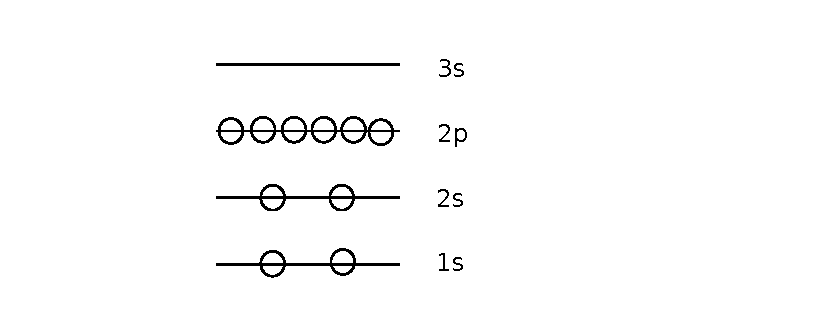
\includegraphics{orbitals.pdf}
  	\caption{Figure showing which hydrogen orbitals are occupied for Neon}
  \end{figure}
  If we disregard the interaction term in the Hamiltonian, this will give the exact result for the system. I have later used this to verify that the code produces the right energies. \par
  For Helium we get
  \begin{align}
  	\Psi_0 = \phi_{1s}(\vec r_1) \phi_{1s}(\vec r_2) \propto e^{-Z(r_1+r_2)} 
  \end{align}
  \begin{align}
  	E_0 = -\frac{Z^2}{2} - \frac{Z^2}{2} = -4
  \end{align}
  While Beryllium gives
  \begin{align}
  	E_{0, Be} = -2\frac{Z^2}{2} - 2 \frac{Z^2}{8} = -16 - 4 = -20
  \end{align}
  And ground state energy for Neon is $-200$. \par
  We cannot neglect the interaction between the electrons, so introduce a variational paramater $\alpha$ instead of the charge $Z$ in the exponent. Using the variational principle, we will vary this $\alpha$ until we get the lowest possible energy. 
 \end{subsection}
 \begin{subsection}{The Jastrow factor}
  As we will see later, the hydrogen orbitals is not a very good approximation to the ground state energy. We can take the interraction between the electrons into account in the wavefunction. This corrolation factor is known as the Padé-Jastrow factor and is on the form
  \begin{align}
  	\Psi_C = \prod_{i<j}^N e^{\frac{ar_{ij}}{1+\beta r_{ij}}}; \quad \quad r_{ij} = \left| \vec r_i - \vec r_j \right| 
  \end{align}
  Here $a=0.25$ if electron $i$ and $j$ have equal spin. Otherwise $a =0.5$. The Jastrow factor accounts for a small amount of the total energy. This is as expected because the interaction between the nucleus and the electrons are much stronger than the electron-electron repulsion. 
 \end{subsection}
 \begin{subsection}{Implemented wavefunctions}
  I have introduced two variational paramaters, namely $\alpha$ and $\beta$. For all three atoms, these are the parametres I will vary until I get the lowest possible energy. \par 
  Helium has two particles only, and splitting the Slater determinant results in two $1x1$ determinants, which can be written without the determinant sign. 
  \begin{align}
  	\Psi_T = \phi_{100 \uparrow}(\vec r_1) \phi_{100 \downarrow}(\vec r_2) \Psi_C(r12) = e^{-\alpha (r1+r2)} \text{exp}(\frac{r_{12}}{2(1+\beta r_{12})})
  \end{align}

  The Beryllium and Neon wave functions iare given by the spin-up and spin-down determinants defined above
  \begin{align}
  	\Psi_T = \text{det}\uparrow(r_1,r_2) \cdot \text{det}\downarrow(r_3,r_4) \prod_{i<j}^N e^{\frac{ar_{ij}}{1+\beta r_{ij}}}
  \end{align}
  where the Neon determinants are $5x5$ matrices given as
  \begin{align}
  	\text{det}\uparrow = \left| \begin{matrix}
	 	\phi_{100 \uparrow} (r_1)  &  \phi_{100 \uparrow} (r_2)  & \phi_{100 \uparrow} (r_3) &  \phi_{100 \uparrow} (r_4) & \phi_{100 \uparrow} (r_5) \\
		\phi_{200 \uparrow} (r_1)  &  \phi_{200 \uparrow} (r_2)  & \phi_{200 \uparrow} (r_3) &  \phi_{200 \uparrow} (r_4) & \phi_{200 \uparrow} (r_5) \\
		\phi_{21-1 \uparrow} (r_1)  &  \phi_{21-1 \uparrow} (r_2)  & \phi_{21-1 \uparrow} (r_3) &  \phi_{21-1 \uparrow} (r_4) & \phi_{21-1 \uparrow} (r_5) \\
		\phi_{210 \uparrow} (r_1)  &  \phi_{210 \uparrow} (r_2)  & \phi_{210 \uparrow} (r_3) &  \phi_{210 \uparrow} (r_4) & \phi_{210 \uparrow} (r_5) \\
		\phi_{211 \uparrow} (r_1)  &  \phi_{211 \uparrow} (r_2)  & \phi_{211 \uparrow} (r_3) &  \phi_{211 \uparrow} (r_4) & \phi_{211 \uparrow} (r_5) \\			
           	     \end{matrix} \right|
  \end{align}
 \end{subsection}

 \begin{subsection}{Gaussian type orbitals}
  Trying and testing for the best $\alpha$ is a crude and unprecise way of finding the optimal parameter. A better method to find the optimal wavefunction is by using a Hartree-Fock calculation. This has been done by someone else, and I have been given the results from dr. Morten Hjorth-Jensen by email. Remember from from the section on Hartree-Fock that we want to expand the wavefunction in a known basis 
  \begin{align*}
 		\left| \phi_p \right> = \sum_\lambda C_{p \lambda} \phi_ \lambda
 	\end{align*}
  And the weights $C_{p \lambda}$ determine wether this is a good approximation or not. The known basis I have used are the GTO and the weights are from the 3-21G basis set. 

  The Gaussian type orbitals are on the form
  \begin{align}
  	G_{ijk}(a,\vec r) = \left( \frac{2a}{\pi}	\right)^{3/4} \left[ \frac{(8a)^{i+j+k} i! j! k! }{(2i)!(2j)!(2k)!} \right] x^i y^j z^k exp(-a r^2)
  \end{align}
  Unfortunatly this does not behave nicely because it does not have the proper exponential decay. We can form a linear combination of them, as we have done in in project two. The main reason why GTO's are a good choice for the basis, is the simplicity when multiplying two different functions. 
  \begin{align}
  	\Xi^{CGTO}(\vec r,i,j,k) = \sum_{p=1}^L d_p G_{ijk}(a_p, \vec r)
  \end{align}
  For Helium this will look like 
  	\begin{align}
  	 \Psi_{He} = K_1 c_1 N_{000} e^{-\alpha_1 r^2} + K_2 \left( c_2 N_{100} e^{-\alpha_2 r^2} + c_3 N_{100} e^{-\alpha_3 r^2} \right)
  	\end{align}
  	where 
  	\begin{align}
  		N_{ijk} = \left( \frac{2a}{\pi}	\right)^{3/4} \left[ \frac{(4a)^{i+j+k} }{(2i-1)!!(2j-1)!!(2k-1)!!} \right] x^i y^j z^k 
  	\end{align}

  And for Beryllium and Neon this will look like
	\begin{align}
	\psi_{Be}&=
	K_{1}\biggl(c_{1}N_{0,0,0}e^{-\alpha_{1}r^{2}}+c_{2}N_{0,0,0}e^{-\alpha_{2}r^{2}}+c_{3}N_{0,0,0}e^{-\alpha_{3}r^{2}}\biggl)\\
	&+K_{2}\biggl(c_{4}N_{0,0,0}e^{-\alpha_{4}r^{2}}+c_{5}N_{0,0,0}e^{-\alpha_{5}r^{2}}\biggl)
	+K_{3}\biggl(c_{6}N_{0,0,0}e^{-\alpha_{6}r^{2}}\biggl)\\
	&+K_{4}\biggl(c_{7}N_{1,0,0}e^{-\alpha_{7}r^{2}}+c_{8}N_{1,0,0}e^{-\alpha_{8}r^{2}}\biggl)
	+K_{5}\biggl(c_{9}N_{1,0,0}e^{-\alpha_{9}r^{2}}\biggl)\\
	&+K_{6}\biggl(c_{7}N_{0,1,0}e^{-\alpha_{7}r^{2}}+c_{8}N_{0,1,0}e^{-\alpha_{8}r^{2}}\biggl)
	+K_{7}\biggl(c_{9}N_{0,1,0}e^{-\alpha_{9}r^{2}}\biggl)\\
	&+K_{8}\biggl(c_{7}N_{0,0,1}e^{-\alpha_{7}r^{2}}+c_{8}N_{0,0,1}e^{-\alpha_{8}r^{2}}\biggl)
	+K_{9}\biggl(c_{9}N_{0,0,1}e^{-\alpha_{9}r^{2}}\biggl)
	\end{align}
  For Beryllium and Neon I get more than one of each of the $K_i's$. This is because each row in the split Slater determinant needs it's own $K_i$. 
 \end{subsection}
\end{section}
\newpage









\begin{section}{Variational Monte Carlo method}
   et teori avsnitt hvor du skriver kort om hva slags teorielement du har brukt (variasjonell MC, statistisk analyse med blocking, gradient metoder og soeking etter minima og mer), deretter

   As stated in the introduction, the point of the project is to solve the Schrodinger equation and find the ground state energy
   \begin{align}
   	\hat H \left| \Psi \right> = E \left|\Psi \right> 
   \end{align}
   This will be done by taking the expectation value of the Hamiltonian
   \begin{align}
   	\left< \Psi \right| \hat H \left| \Psi \right> = E[H] = \frac{\int d \mathbf{R} \Psi^*_T(\mathbf{R}) H(\mathbf{R}) \Psi_T(\mathbf{R})}{ \int d \mathbf{R} \Psi^*_T(\mathbf{R}) \Psi_T(\mathbf{R})}
   \end{align}
 	And from the variational principle, we know that 
 	\begin{align}
 		E[H] \geq E_{gs}
 	\end{align}
 	So the steps of this project is to choose a variational wavefunction, calculate the integral for $E[H]$ and minimize it with respect to the variational parametres. That is, we need to minimize the value
 	\begin{align}
 		E[H(\alpha, \beta)] = \frac{\int d \mathbf{R} \Psi^*_T(\mathbf{R},\alpha,\beta) H(\mathbf{R}) \Psi_T(\mathbf{R},\alpha,\beta)}{ \int d \mathbf{R} \Psi^*_T(\mathbf{R},\alpha,\beta) \Psi_T(\mathbf{R},\alpha,\beta)}
 	\end{align}
 	We define a new quatnity 
 	\begin{align}
 		E_L({\mathbf{R},\alpha,\beta}) = \frac{1}{\Psi_T(\mathbf{R},\alpha,\beta)} \hat H \Psi(\mathbf{R},\alpha,\beta)
 	\end{align}
 	And we see that by introducing the probability distribution
 	\begin{align}
 		P(\mathbf{R}) = \frac{|\Psi(\mathbf{R})|^2}{\int|\Psi(\mathbf{R})|^2 d \mathbf{R}}
 	\end{align}
 	We can write the total energy as
 	\begin{align}
 		E[H(\alpha,\beta)] = \int P(\mathbf{R},\alpha,\beta) E_(\mathbf{R},\alpha,\beta) d \mathbf{R} \approx \frac{1}{N} \sum_{i=1}^N P(\mathbf{R}_i,\alpha,\beta) E_L(\mathbf{R}_i,\alpha,\beta)
 	\end{align}
 	Where we calculate the local energy in each time and take the mean value. 

 \begin{subsection}{Metropolis algorithm}
 	The metropolis algorithm is a way to incorporate the probability distribution function in the calculation. The Metropolis algorithm is defined as following. We define $P_i^n$ as the probability of finding the system in the state $i$ at the step n. 
 	We now sample a possible new state $j$ with the probability $T_{i\to j}$. 

 	There is a probability $A_{i\to j}$ that we accept this new state, and $1-A_{i \to j}$ probability that we reject the move and use state $i$ again. 

 	We can show that 
	\begin{align}
 		\frac{A_{j\to i}}{A_{i\to j}} = \frac{p_i T_{i\to j}}{p_j T_{j\to i}}	
 	\end{align}
 	And the Metropolis choice is to maximize the A values, i.e. 
 	\begin{align}
 		A_{j \to i} = min\left( 1, \frac{p_i T_{i\to j}}{p_j T_{j\to i}} \right)
 	\end{align}
 	The factor 
 	\begin{align}
 		\frac{p_i T_{i\to j}}{p_j T_{j\to i}} = \frac{|\Psi_T(R_{new})|^2}{\Psi_T(R_{old})|^2}
 	\end{align}

 	This will make sure that we integrate over the positions multiplied with the corresponding probability distribution, $P(\mathbf{R})$. 


 \end{subsection}

 \begin{subsection}{Importance sampling}
 	The metropolis algorithm is a brute force implementation of the probability distribution. We can replace it with a walk in coordinate space biased by the trial wave function. That is a walk influenced by the forces acting on the particle. 
 	For a diffusion process characterized by a time-dependent probability density $P(x,t)$ the Fokker-Planck equation reads
 	\begin{align}
 		\frac{\partial P}{\partial t} = D \frac{\partial }{\partial x} \left( \frac{\partial}{\partial x} - F \right) P(x,t)
 	\end{align}
 	We use Euler's method to find solutions to this problem. The new position reads
 	\begin{align}
 		y = x + DF(x) \Delta t + \xi \sqrt(\Delta t)
 	\end{align}
 	where $\xi$ is a random variable and $\Delta t$ is a chosen time step. I will investigate which time steps give stable results. $D = \frac{1}{2}$ because of the factor in the kinetic energy operator. \par
 	The force is calculated by
 	\begin{align}
 		\mathbf{F} = 2 \frac{1}{\Psi_T}\nabla \Psi_T 
 	\end{align}
 	The transition probability must be changed aswell. the general Metropolis algorithm reads
 	\begin{align}
 		A_{y,x} = min \left(1, q(y,x) \right)
 	\end{align}
 	but now we replace $q(y,x) = \frac{|\Psi_T(R_{new})|^2}{\Psi_T(R_{old})|^2}$ with
 	\begin{align}
 		q(y,x) = \frac{G(x,y,\Delta t)|\Psi_T(y)|^2}{G(y,x,\Delta t)|\Psi_T(x)|^2}
 	\end{align}
 	where we have introduced the Green's function
 	\begin{align}
 		G(y,x,\Delta t) \propto exp(-(y-x-D\Delta t F(x))^2 / 4D\Delta t)
 	\end{align}
 \end{subsection}

 \begin{subsection}{Statistical analysis}
 	A Monte Carlo simulation gives rise to two kinds of error. Systematic errors and statistical errors. Systematic errors are due to limitations of the applied models and faulty implementations. Here I will explore methods to estimate the statistical error. 

 Given a set of local energies, the variance is a measure of the spread from the true mean. The definition is
 \begin{align*}
 	\text{Var}(E) = \left< E^2 \right> - \left< E \right> ^2 
 \end{align*}
 Unfortunatly we do not know the true mean in a Monte-Carlo simulation. The computed average $\overline E$ is an approximation to the exact mean, and we do the following approximation
 \begin{align*}
 	\text{Var}(E) \approx \overline{E^2} - \overline{E}^2 
 \end{align*}
 For the case where we have the exact wave function, the variance becomes $0$, so the variance is an excellent measure of how close we are to the exact wave function. The variance however is \textit{not} a direct measure of the error. The standard deviation, the square root of the variance is related of the \textit{spread} in the sampled value. 
 \begin{align}
 	\sigma ^2(x) = \text{Var}(x)
 	\label{deviation}
 \end{align}
 This does not account for the samples being corrolated. Two samples, $x$ and $y$ are corrolated if the \textit{Covariance} is non-zero.
 \begin{align*}
 	\text{Cov}(x,y) = \left< xy \right> - \left< x \right> \left<y \right> 
 \end{align*}
 The diagonal elements of the Covariance is the Variance. By ignoring the corrolations, one get an error estimate that is generally too small. Given the true deviation, $\sigma_e$ and $\sigma$ from (\ref{deviation}) we have
 \begin{align*}
 	\sigma_c \geq \sigma
 \end{align*}

 The most interesting quantity when doing statistical analysis is not the error of single samples. It is the error of the mean value. One can show that the variance for the mean value, $m$ is 
 \begin{align}
 	\sigma^2 (m) = \frac{1}{n} \text{Cov}(x)
 	\label{covariance}
 \end{align}
 Where n is the number of samples used to calculate $m$ and 
 \begin{align*}
 	m = \frac{1}{n} \sum_i^n x_i
 \end{align*}
 Calculating the Covariance is an expensive process for a large sample set, so we need a better way to calculate this. 

 There is no need to do statistical analysis within the Monte-Carlo simulation. By storing the data set, one can estimate the error post process. An efficient algorithm for this is called blocking. 

 Given a set of $N$ samples from a single Monte-Carlo process. This set is divided into $n$ blocks of size $n_b = N/n$. Now we can treat each block as an individual simulation to calculate the variance of a calculated mean, $m$. This will in turn give us the covariance by (\ref{covariance}).
 \begin{align*}
 	\sigma^2 (m) = \left<m^2\right> - \left<m\right>^2 
 \end{align*}

 One can not know beforehand which block size is optimal to compute the exact error. One can, however, plot the variance against different block sizes. The curve should be stable over a span of block sizes. This plateau will serve as a reasonable approximation to the covariance. 
 \end{subsection}
 \begin{subsection}{One-body density}
 	The one-body density is defined as
 \begin{align*}
 	\rho(r_1) = \int_{r_2} .. \int_{r_N} | \Phi(r_1 r_2 .. r_N) |^2 dr_2 .. dr_N
 \end{align*}

 The distribution $|\Phi(r)|^2$ describes the distribution of a particle in the system. The one-body density $\rho(r_1)$ describes the simultaneous distribution of every particle in the system. $\rho(r_1) dr_1 $ represents the probability of finding \textit{any} particle in the volume element $dr_1$ as oppsed to $|\Phi(r)|^2$ giving the probability of finding \textit{particle $r_1$} in the volume element $dr_1$. Due to the indistinguishable nature of the particles, any of the coordinates contain information about all the particles. I will therefore normalize this density to the number of particles $N$ and not $1$ which is common for the one-particle density. 

 The way this is computed in a Monte Carlo simulation is by taking snapshots of all positions for every timestep, then constructing a histogram to construct an approximation to the wave function.

 The charge density for a single particle is given by 
 \begin{align*}
 	\rho_q (r) = q |\Psi(r)|^2
 \end{align*}
 However, since we already have computed the many-body probability density, we can use this instead to get the many-body charge density of the system. 
 \begin{align*}
 	\rho_q (r) = Q \rho(r_1)
 \end{align*}
 \end{subsection}

 \begin{subsection}{Method of steepest descent}
  	Up until now, I have used measurment by eye to find the optimal values for $\alpha$ and $\beta$. This can be done in a more precise way, namely using methods like steepest descent or Conjugate Gradient method. I have included the steepest descent method in my project.
 If a function $F(x)$ is differentiable and in the neighborhood of a point $\mathbf{a}$, then the function $F(x)$ decreases fastest in the direction of the negative gradient, $-\nabla F(x)$. i.e. we are approaching a minima. Since the variational principle holds for $\left<\hat H\right> $, the best values for $\alpha$ and $\beta$ are the ones giving this minima. 
 \begin{align*}
 	\mathbf{b} = \mathbf{a} - \gamma \nabla F(\mathbf{a}) 
 \end{align*}
 if $\gamma$ is small enough, $F(\mathbf{b}) \leq F(\mathbf{a})$. We can therefore set up the scheme
 \begin{align*}
 	x_{n+1} = x_n - \gamma \nabla F(x_n)
 \end{align*}
 and continue until
 \begin{align*}
 	x_{n+1} - x_n \leq \text{precision}
 \end{align*}
  \end{subsection}

\end{section}
\newpage













\begin{section}{Implementation}
  * et implementasjon kapittel hvor du forteller hvordan du har implementert teorien, skriv om algo for SD, algo for Jastrow faktor, hvordan blocking er implementert samt testen du har brukt for aa verifisere koden. Her boer du baade diskutere hvordan du har testa analytisk lokal energi kontra numerisk derivasjon, liste cpu tidsbesparelse samt andre tester du har gjort, feks analytisk SD for beryllium kontra algoritmen for beryllium osv. Du trenger ikke liste heile koden her, det kan du legge til appendiks. 

  The general algorithm which is implemented for the variational monte carlo simulation goes as


 \begin{subsection}{Slater determinant}
 	The way I have implemented the Slater determinant is by having two smaller determinants for spin up and spin down. That means I only need to update one of the determinants when after accepting a move. When I calculate the local energy and quantum force, I will need the inverse of the determinatn. This is a costly operation, so instead of computing the inverse for every time-step, we can use the following algorithm to update inverse matrix elements for each step. 
 	\begin{align}
 		d_{kj}^{-1}(\mathbf{x^{new}}) = \left\{
	\begin{array}{ll}
		d_{kj}^{-1}(\mathbf{x}^{old}) - \frac{d_{kj}^{-1}(\mathbf{x}^{old})}{R} \sum_{l=1}^N d_{il}(\mathbf{x}^{new})d_{il}^{-1}(\mathbf{x}^{old})  & \mbox{if } j \neq i \\
		\frac{d_{kj}^{-1}(\mathbf{x}^{old})}{R} \sum_{l=1}^N d_{il}(\mathbf{x}^{old})d_{il}^{-1}(\mathbf{x}^{old}) & \mbox{if } j = i
	\end{array}
	\right.
 	\end{align}
 	This can save some computation time. 
 \end{subsection}

 \begin{subsection}{Closed form expression for local energy and quantum force}
 	See appendix A for derivation of the closed form expression for Helium. On the general form we have the closed form expression
 	\begin{align}
 		\frac{\nabla^2 \Psi}{\Psi} = \frac{\nabla^2_i|\hat D(\mathbf{r})|}{|\hat D(\mathbf{r})|} + \frac{\nabla^2 \Psi_C}{\Psi_C} + 2 \frac{\nabla_i|\hat D(\mathbf{r})|}{|\hat D(\mathbf{r})|} \cdot \frac{\nabla_k \Psi_C}{\Psi_C}
 	\end{align}
 	When we calculate the gradient and Laplacian we use the following formulas
 	\begin{align}
 		\frac{\nabla_i|\hat D(\mathbf{r})|}{|\hat D(\mathbf{r})|} &= \sum_{j=1}^N \nabla_i d_{ij}(\mathbf{r})d_{ji}^{-1} \\
 		\frac{\nabla^2_i|\hat D(\mathbf{r})|}{|\hat D(\mathbf{r})|} &= \sum_{j=1}^N \nabla^2_i d_{ij}(\mathbf{r})d_{ji}^{-1} 
 	\end{align}
 	And the following are used for the Jastrow factor
 	\begin{align*}
 		\frac{\nabla_k \Psi_C}{\Psi_C} = &\sum_{j\neq k} \frac{\mathbf{r}_{kj}}{r_{kj}} \frac{a}{(1+\beta r_{kj})^2}
 		\frac{\nabla_k^2 \Psi_C}{\Psi_C} = \sum_{ij \neq k} \frac{(\mathbf{r}_k - \mathbf{r}_i) \cdot (\mathbf{r}_k - \mathbf{r}_j)}{r_{ki}r_{kj}} \frac{a}{(1+\beta r_ki)^2} \frac{a}{(1+\beta r_kj)^2} \\ + &\sum_{j\neq k} \left( \frac{2a}{r_{kj}(1+\beta r_{kj})^2} - \frac{2a \beta}{(1 + \beta r_{kj}})^3 \right)
 	\end{align*}
 \end{subsection}

 \begin{subsection}{Finding optimal step length}
  In the Metropolis algorithm without importance sampling, we need a steplength. An optimal step length has an acceptance rate around $50\%$, so I measured how many moves were accepted and calculated the mean value. If the amount of accepted moves were too far from $50\%$, I changed the step length and ran the code again. This is found in the function \textit{void VMCSolver::MCintegration\_FindVariables}. 
  This is the same code that was used to find the optimal $\beta$ in the Steepest descent method. 
 \end{subsection}
	
 \begin{subsection}{Parallell programming}
  One of the most powerfull optimization tools is parallell programming. We can run one parallell thread on each core, and can with $4$ cores on my computer use $4$ times as many time steps. Variational monte carlo is easy to parallellize. We can make each core do $N$ samples with a specified random seed, and take the mean of each result. \par
  I use the function \textit{MPI\_Reduce} to gather all the calculated information into one of the processors. Then that processor will calculate means, variance and write the result out to file. 
 \end{subsection}

 \begin{subsection}{Problems when implementing the code}
  There have been a few problems with this code. I did not get everything to work proberly for Neon and Beryllium. For Helium everything works as intended. I get the exact same result using the closed form expressions for local energy and quantum force as I do when I use the numerically calculated values. For Beryllium, the closed form expressions for energy gives almost the same result, but the Quantum force crashed completely with the closed form expression. As for Neon, only the numerical calculations gives anything close to the expected values. I have, when looking at the results for Neon og Beryllium, used numerically calculated energies.

  There are a few problems with the method of steepest descent as well. For Helium it seems to converge towards a reasonable $\beta$, but for Beryllium and Neon, the difference in energy due to a change in $\beta$ is so small that the method does not manage to converge against the optimal value. It merely stays put if I give it a reasonably initial guess. 
 \end{subsection}

\end{section}
 \newpage









\begin{section}{Results and discussion}

* resultater. Her kan du diskutere bla resultatene for He, be og Ne med de ulike approksimasjonene du har gjort, rekninger med bare SD og rekninger med baade SD og Jastrow. Hvor mye paavirker Jastrow faktoren resultatet for energien, er det forskjeller mellom He, be og Ne med tanke paa korrelasjoner, dvs spiller Jastrow faktoren like stor rolle for alle tre atomer osv. I tillegg boer du diskutere jastrow faktorens rolle naar du plotter en-partikkeltettheter og proeve aa trekke noen konklusjoner utifra det.


 \begin{subsection}{First look at Helium atom}
 	The first attempt at finding the ground state energy for Helium is found in the code for Project 1. figure (\ref{Helium1}) shows the variance and energy as we vary the parameter alpha. These results are without the Jastrow factor. 

 \begin{figure}[H]
 	\centering
 	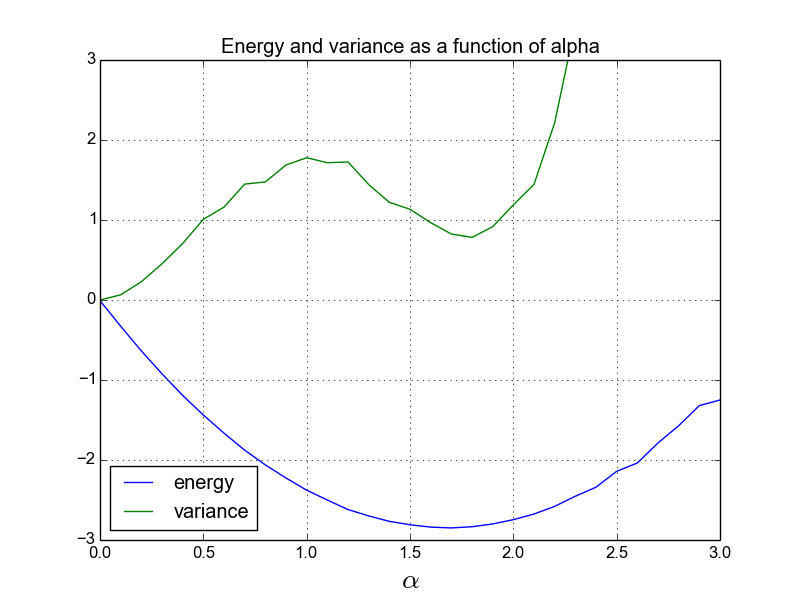
\includegraphics[width=0.8\textwidth]{../python_programs/EnergyVariance_helium1.png}
 	\label{Helium1}
 	\caption{A plot of the ground state energy for Helium for as a function of different $\alpha$ values. This has been calculated with Jastrow factor, Hydrogen-like orbitals and Steepest descent to find $\beta$. The corresponding variance has been included in the plot. }
 \end{figure}

 By looking closer at the energy and variance around $\alpha = 1.68$ in figure (\ref{Helium2}), we see that we get an energy of $\left<E\right> = -2.84997$, with a variance of $\sigma ^2 = 0.932912$. This is too far off from the best experimental value of $E_{experimental} = -2.903$. We see however that the variance is smaller for $\alpha = 1.8$, $1.9$ and $1.6$. But by the variational principle, we want as low energy as possible, so we choose the best $\alpha$ as $1.68$. 
 
 \begin{figure}[H]
 	\centering
 	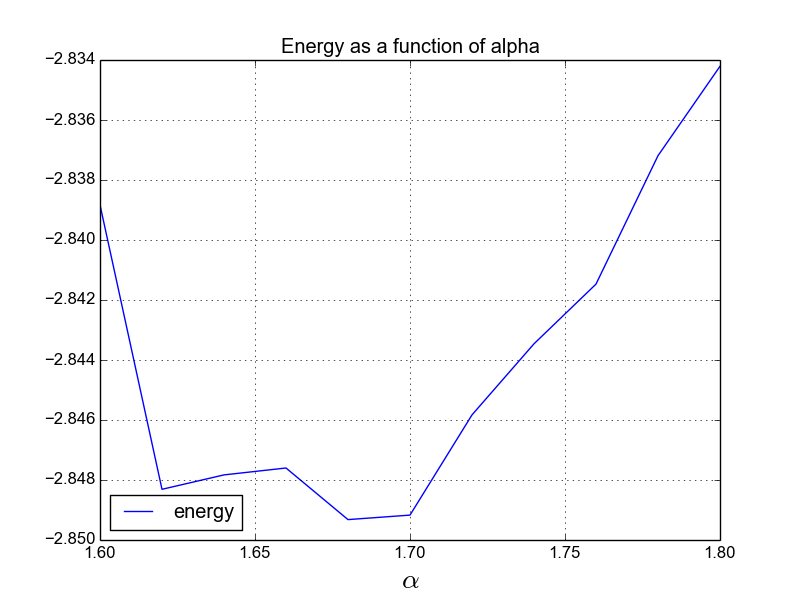
\includegraphics[width=0.8\textwidth]{../python_programs/EnergyVariance_helium2.png}
 	\label{Helium2}
	\caption{A closer look at which $\alpha$'s give the lowest $E_{gs}$}
 \end{figure}

 We now use Importance sampling in our calculations to look at which dt's are stable. 
 We can see from the plot below that using $dt = 10^-3$, we get stable results. A smaller $dt$ probably gives rise to different kinds of errors, like truncation errors etc.  
 \begin{figure}[H] 
 	\centering
 	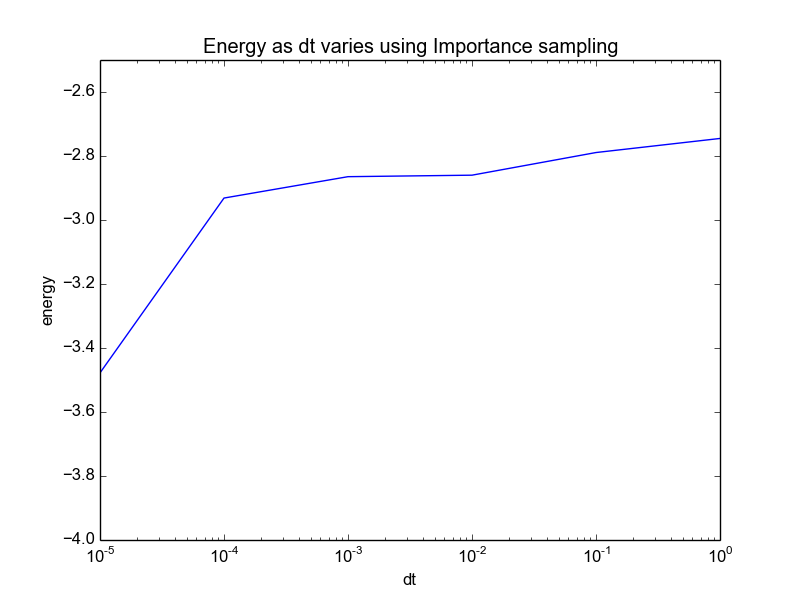
\includegraphics[width=0.8\textwidth]{../python_programs/ImportanceSampling_Helium_dt.png}
 	\caption{Shows a plot of the ground state energy calculated with importance sampling for different values of $\Delta t$. We see that we get stable values around $10^{-1}$ and $10^{-3}$. }
 \end{figure}

 We can also look at the effect of including the Jastrow factor. In the plot below, we see that we get noticably lower energies; Around $E = -2.89207$ for the optimal values of $\alpha$ and $\beta$. This plot does a poor job of representing which $\beta$ is optimal, but from now on, I will use the Steepest descent method to find the best $\beta$, so I will not use measurment by eyes to determine the beta. The best value I found in this plot was $\beta = 0.3$. 
 \begin{figure}[H]
 	\centering
 	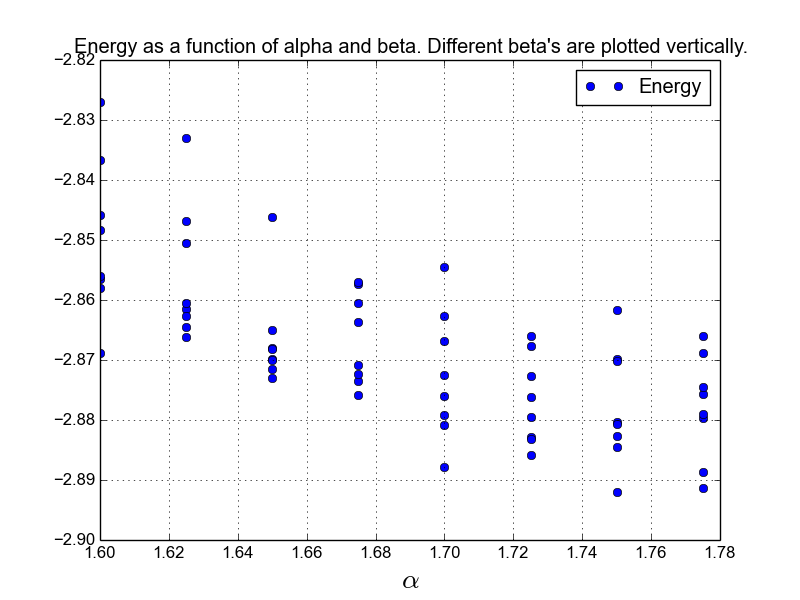
\includegraphics[width=0.8\textwidth]{../python_programs/EnergyVariance_helium5.png}
 	\label{Helium3}
 	\caption{Plotting energy as a function of $\alpha$ by testing some different $\beta$ values for each $\alpha$}
 \end{figure}

 \end{subsection}
 \begin{subsection}{The Helium atom}
 	By excluding the Jastrow factor and the two-body potential in the local energy, one can test wether the Slater determinant is set up right. By setting $\alpha$ equal to the number of particles, one should get $E_0 = -4$. This can be reproduced, both with the analytical local energy, the numerical local energy, the numerical quantum force and the analytical quantum force. After doing these naive simulations, I include the Jastrow factor and the two-body potential. I will also use the method of steepest descent to find the optimal beta. This code runs in parallell and it is run using Importance sampling. The first results are produced without the Gaussian type orbitals. 

	 A short computation time comparison between the numerical and analytical gradients and Laplacians are found in the files, \textit{Helium\_CompareTime.txt}, \textit{Helium\_CompareTime\_ELnum.txt} and \textit{Helium\_CompareTime\_QFnum.txt}. All of them are done with Importance Sampling. 

	 We see that the results are about the same, but the time needed for the computation is $33$s for analytical, $52,3$s for the numerical local energy and finally $65.4$s for the numerical quantum force. 

	 For the final run on Helium with importance sampling and Steepest descent method using Hydrogen-like orbitals, I set $\alpha = 1.75$ as I have seen that this alpha gave the lowest energy when the Jastrow factor was included. The steepest descent method stabilized at $\beta = 0.515163$. I used $10^7$ iterations for each core, so a total of $4 \cdot 10^7$ iterations in the calculation. This running is done with the Importance sampling method, so the only variational parameter that is not perfectly optimized is the value for $\alpha$. This can be fixed by including the Gaussian Orbitals which are a result of Hartree-Fock calculations. They do not have a parameter to be varied, and should for that reason give an optimal value. The result from this calculation is found in the file \textit{Helium\_final\_calculation.txt}. The result gained was
	 \begin{align*}
	 	E = -2.88538
	 \end{align*}

    Switching from Hydrogen-like orbitals to Gaussian type orbitals, I run the code in Project3\_Gaussian. This has been run with and without the Jastrow factor, but with importance sampling and steepest descent to find $\beta$. The results can be displayed in the following table
    
	\begin{center}
	  \begin{tabular}{ l | c | c | c | r }
	    $\beta$ & $E_{vmc}$ & $E_{vmc,JF}$ & $E_{exact}$ & \text{variance w/JF} \\ \hline
	    $0.313749$ & $-2.79024$ & $-2.85517$ & $-2.90037$ & 4.11203 \\ 
	    \hline
	  \end{tabular}
	\end{center}
	We see from this table that the correction from Jastrow factor is really important for Helium. We can make a plot of the radial distribution for the cases with and without the Jastrow factor. 
	
	\begin{figure}[H]
 	\centering
 	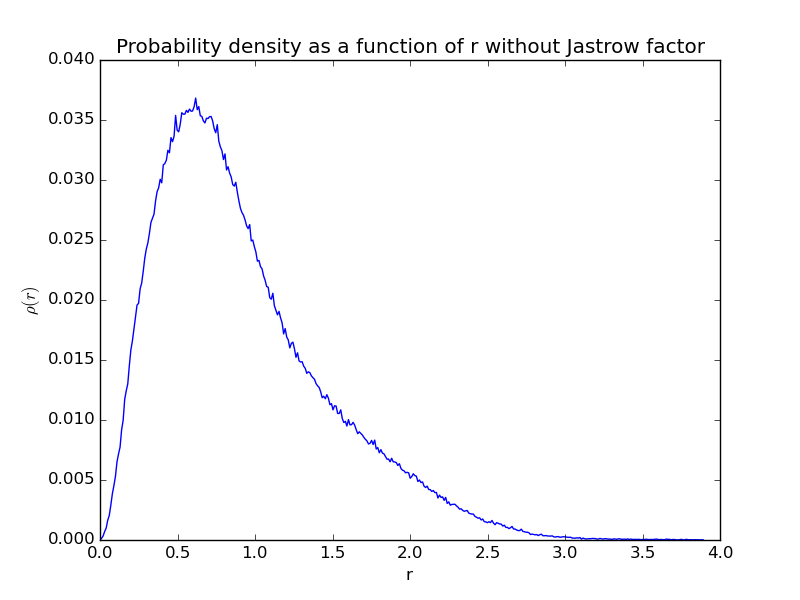
\includegraphics[width=0.8\textwidth]{../../Project3_Gaussian/python_scripts/ProbabilityDensityHelium_Jastrow.png}
 	\label{fig1}
 	\caption{Shows the probability of finding an atom a radius $r$ away from the nucleus. This is with the Jastrow factor}
 	\end{figure}
 	\begin{figure}[H]
 	\centering
 	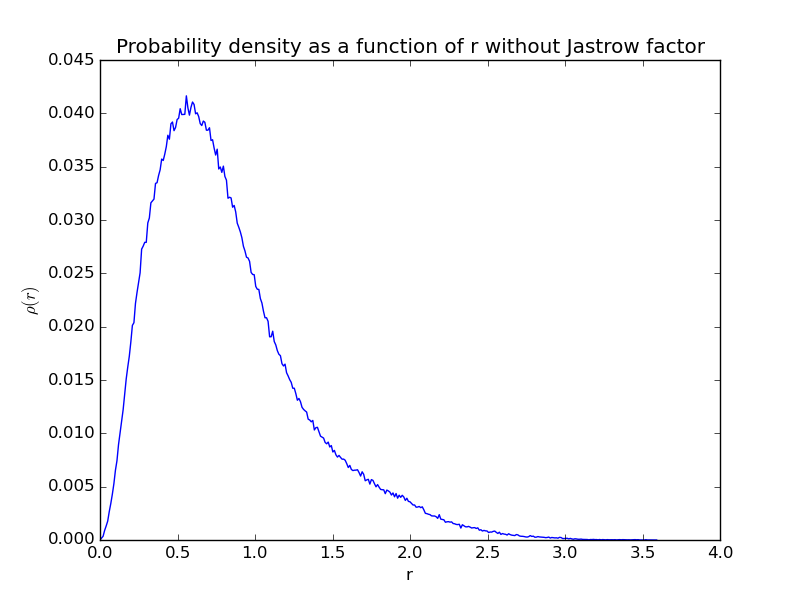
\includegraphics[width=0.8\textwidth]{../../Project3_Gaussian/python_scripts/ProbabilityDensityHelium_noJastrow.png}
 	\caption{Shows the probability of finding an atom a radius $r$ away from the nucleus. This is without the Jastrow factor, and compared to (\ref{fig1}), we see that the electrons are closer to the nucleus without the electron-electron repulsion taken into account.}
 	\end{figure}
 	We see that the electrons are further from the core if we take the Jastrow factor into account. A plot of the the blocking analysis show
 	\begin{figure}[H]
 	\centering
 	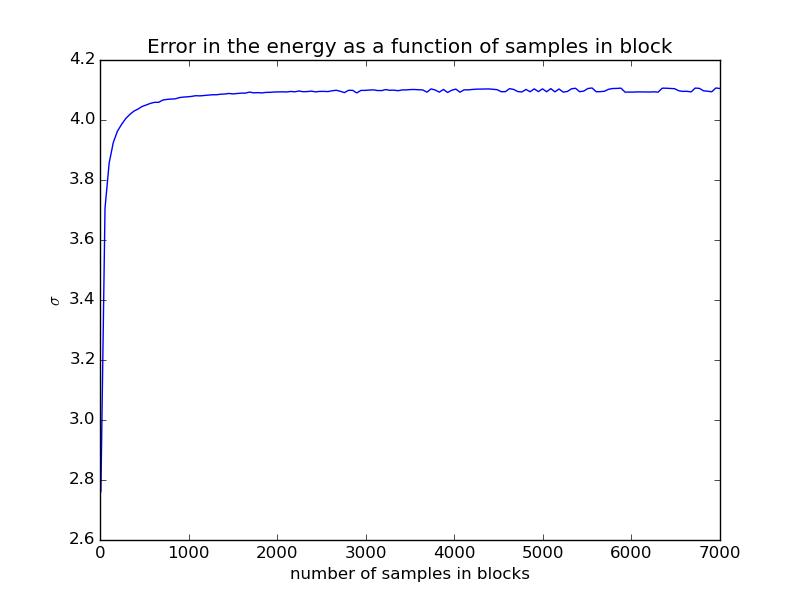
\includegraphics[width=0.8\textwidth]{../../Project3_Gaussian/python_scripts/HeliumBlocking.png}
 	\caption{Shows the variance as a function of samples in a block. We can read of the error where the function has stabilized. Around $4.1$. However the values in this plot is probably wrong, because one would expect much smaller error.}
 	\end{figure}
 	Unfortunatly this plot suggests that I have not managed to calculate the variance correctly for the different block-sizes. I would expect the variance to be much smaller. 


 \end{subsection}
 \begin{subsection}{The Beryllium atom}
 	Removing the repulsion from the potential energy, I get $E = -20$, which is expected. Adding the repulsion and Jastrow factor, I have did a variational Monte Carlo for Helium with hydrogen-like orbitals. 
 	Using the code in project 3 to do calculations on Beryllium I search for a good value of $\alpha$. Looping through 20 different $\alpha$'s from 3 to 4.
 \begin{figure}[H]
 	\centering
 	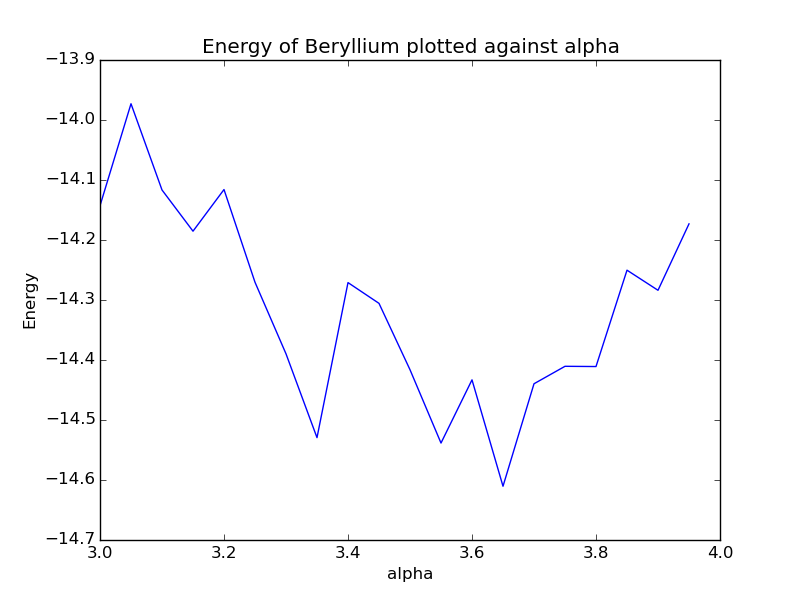
\includegraphics[width=0.8\textwidth]{../python_programs/FindOptimalAlphaBeryllium.png}
 	\caption{A plot of the ground state energy for Beryllium for as a function of different $\alpha$ values. This has been calculated with Jastrow factor, Hydrogen-like orbitals and Steepest descent to find $\beta$}
 \end{figure}
 As seen in the figure, setting $\alpha = 3.65$ gives the lowest energy. A monte carlo integration with that alpha gives 
 \begin{align*}
 	E = -14.4144
 \end{align*}
 with $10^6$ iterations per core. The result is in the file \textit{Beryllium\_MC.txt}. 

 Switching to Gaussian type orbitals to produce the final results, I produce the results
 \begin{center}
	  \begin{tabular}{ l | c | c | c | r }
	    $\beta$ & $E_{vmc}$ & $E_{vmc,JF}$ & $E_{exact}$ & \text{variance w/JF} \\ \hline
	    $0.6$ & $-14.5338$ & $-14.3394$ & $-14.667$ & 33.0956 \\ 
	    \hline
 \end{tabular} 
 \end{center}
 Surprisingly I get better results without the Jastrow factor for Beryllium. A plot of the radial distribution of particles for Beryllium 

 \begin{figure}[H]
 	\centering
 	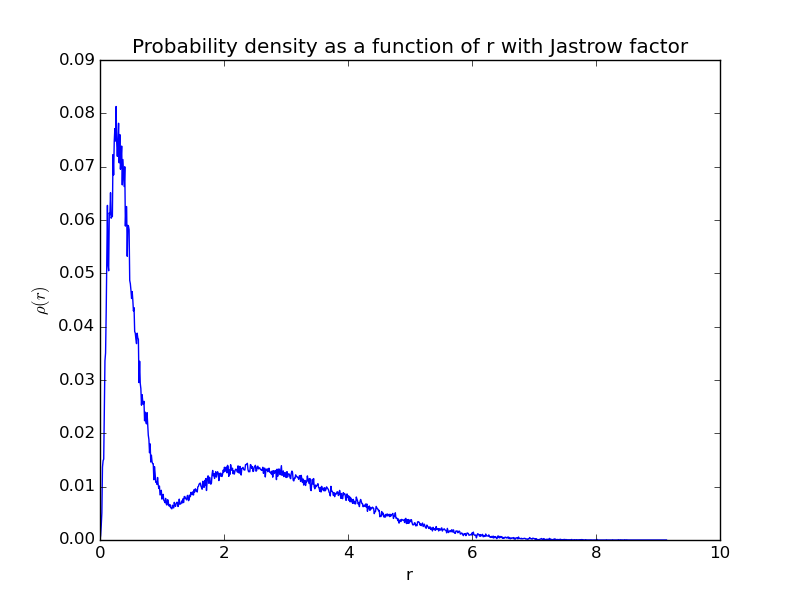
\includegraphics[width=0.8\textwidth]{../../Project3_Gaussian/python_scripts/ProbabilityDensityBeryllium_Jastrow.png}
 	\caption{Shows the probability of finding an atom a radius $r$ away from the nucleus. This is with the Jastrow factor. Notice that we see the 2s-orbitals as the second \textit{bump}}
 \end{figure}

 \end{subsection}

 \begin{subsection}{The Neon atom}
  First I have made a plot of the energy as a function of $\alpha$. This plot is made with the Jastrow factor and with Hydrogen orbitals. 
  \begin{figure}[H]
 	\centering
 	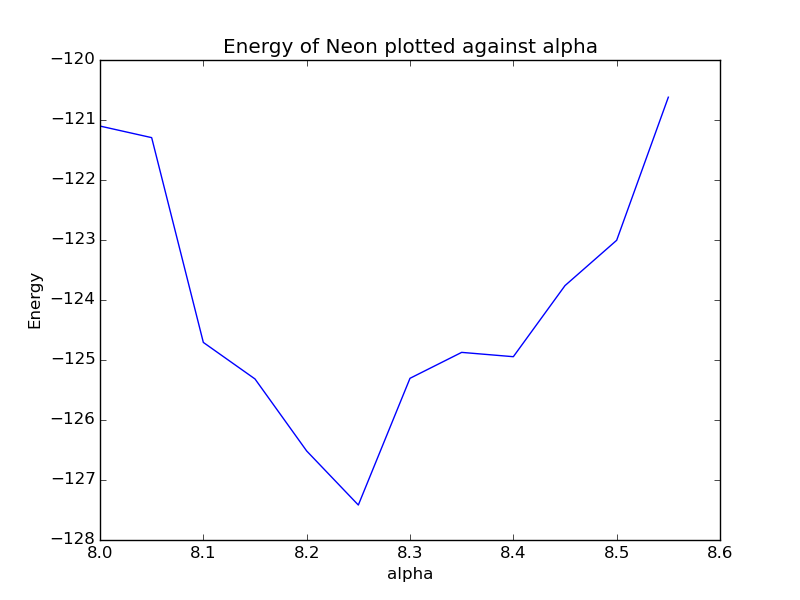
\includegraphics[width=0.8\textwidth]{../python_programs/FindOptimalAlphaNeon.png}
 	\caption{A plot of the ground state energy of Neon for as a function of different $\alpha$ values. This has been calculated with Jastrow factor, Hydrogen-like orbitals and Steepest descent to find $\beta$}
 \end{figure}
 We see that an $\alpha$ close to $8.25$ gives an energy very close to the experimental value of $-128.94$.

 Introducing Gaussian-type orbitals we get the results 
 \begin{center}
	  \begin{tabular}{ l | c | c | c | r }
	    $\beta$ & $E_{vmc}$ & $E_{vmc,JF}$ & $E_{exact}$ & \text{variance w/JF} \\ \hline
	    $0.6$ & $-124.875$ & $-124.875$ & $-128.94$ & 349.915 \\ 
	    \hline
 \end{tabular} 
 \end{center}
 As with the Helium and Beryllium atoms, I plot the probability density and I see that the particles are spread more evenly out, with most of them occupying the 2p-states furthest away from the center. 
 \begin{figure}[H]
 	\centering
 	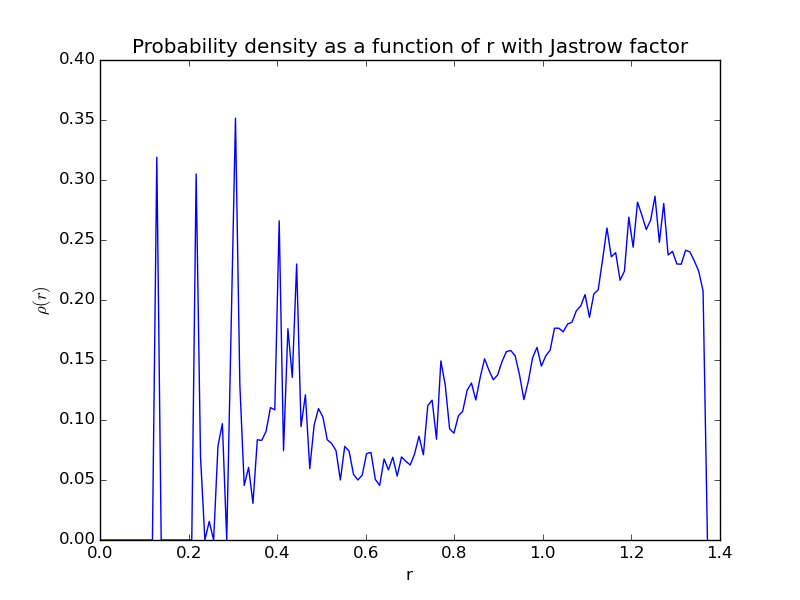
\includegraphics[width=0.8\textwidth]{../../Project3_Gaussian/python_scripts/ProbabilityDensityNeon_Jastrow.png}
 	\caption{Shows the probability of finding an atom a radius $r$ away from the nucleus. This is with the Jastrow factor. Here the particles are starting to spread very evenly out. The plot could be nicer close to $r=0$ with more samples.}
 \end{figure}
 \end{subsection}
\end{section}
\newpage








\begin{section}{Conclusion}
 This has been a very interesting project. I have looked closely at different methods of finding the ground state energy for different atoms. The \textit{brute force} method of using hydrogen-like orbitals without a Jastrow factor did actually produce relatively good approximations. For chemistry, we require a much better approximation to the energy, and we introduced the Jastrow factor to achieve this. I do, however, not believe that this correction is enough to look at chemical properties of the atoms, so there are probably even better methods one can use. I saw also that the Jastrow factor was most important for the smaller atoms. \par
 Introducing the GTO's instead of Hydrogen-like orbitals, the point was to fix the variational parameter in the Slater determinant. I did however not get as good results for these basis functions. I do not know why. I did not manage to find an error in the implementation, and the results for Neon shows that my code cannot be terribly wrong. \par
 There are some small details that I never managed to implement properly. As stated earlier, the program worked perfectly for Helium, but some small problems came around for Beryllium and Neon. As well as a problem with the blocking analysis. This really bugs me, but I do no longer have time to fix this properly. This is the largest code I have written, and it grew in every direction as I wanted to add a new feature. This made it harder and harder to fully comprehend what was going on. This is probably a valuable lesson I will be grateful for in the future. Maybe. \par
 Overall I have enjoyed the course even though it has been the most demanding course I have taken. 
\end{section}
 
 \begin{section}{Sources}
  \begin{itemize}
  	\item Lecture Notes from FYS4411 2015
  	\item Håvard Tveit Ihle's project from 2013
  	\item Jørgen Høgberget Master Thesis
  	\item I have cooperated with Alexander Fleischer and Daniel Bjørnstad on some small matters
  \end{itemize}
 \end{section}

\newpage









\appendix
\begin{section}{Appendix A}

\begin{subsection}{Analytical calculation of the local energy}
 Calculating the kinetic energy numerically is costly. One can considerably reduce computational time by using a closed form expression for the energy. 

 We have trial wavefunction 
 \begin{align*}
 	\Psi = e^{-\alpha(r_1 + r_2)}
 \end{align*}
 and we want to calculate the local energy given by
 \begin{align*}
 	E_L = \frac{1}{\Psi} \hat H \Psi
 \end{align*}
 where
 \begin{align*}
 	\hat H = -\frac{\nabla_1^2}{2} - \frac{\nabla_2^2}{2} - \frac{2}{r_1} - \frac{2}{r_2} + \frac{1}{r_{12}}
 \end{align*}
 Rewriting	
 \begin{align*}
 	T_{L1} = \frac{1}{\Psi} \left( -\frac{\nabla_1^2}{2} - \frac{\nabla_2^2}{2} \right) \Psi
 \end{align*}
 \begin{align*}
 	V_{L1} = \frac{1}{\Psi} \left( - \frac{2}{r_1} - \frac{2}{r_2} + \frac{1}{r_{12}} \right) \Psi
 \end{align*}
 Doing the calculations, we find that
 \begin{align*}
 	T_{L1} = -\frac{1}{2} \frac{1}{\Psi} \left( \frac{1}{r_1^2} \frac{\partial}{\partial r_1} \left( r_1^2 \frac{\partial}{\partial r_1} \Psi \right) + \frac{1}{r_2^2} \frac{\partial}{\partial r_2} \left( r_2^2 \frac{\partial}{\partial r_2} \Psi \right) \right)
 \end{align*}
 \begin{align*}
 	T_{L1} = -\frac{1}{2} \left( -\frac{2}{r_1}\alpha + \alpha^2 - \frac{2}{r_2} + \alpha^2 \right)
 \end{align*}
 Adding $T_{L1}$ and $V_{L1}$ 
 \begin{align*}
 	E_{L1} = \left( \alpha - 2 \right) \left( \frac{1}{r_1} + \frac{1}{r_2} \right) + \frac{1}{r_{12}} - \alpha^2 
 \end{align*}

 Introducing the Jastrow factor, one can rewrite the wavefunction
 as a product of the direct term and the corrolation term. 
 \begin{align*}
 	\Psi = \Psi_D \Psi_C
 \end{align*}
 We want to calculate the kinetic energy and divide by the wavefunction.
 \begin{align*}
 	T_{L2} = \frac{1}{\Psi} \frac{-\nabla^2}{2} \Psi
 \end{align*}
 Using the chain rule. This equation must be calculated for both particles. 
 \begin{align}
 	T_{L2} = -\frac{1}{2} \left( \frac{1}{\Psi_D}\nabla^2 \Psi_D + 2 \frac{1}{\Psi_D \Psi_C} \nabla \Psi_D \cdot \nabla \Psi_C + \nabla^2 \Psi_C \right)
 	\label{T_L2}
 \end{align}
 The first term is easily calculated, as it is the same as for $E_{L1}$
 \begin{align*}
 	\frac{1}{\Psi_D}\nabla^2 \Psi_D =  -\frac{2}{r_1}\alpha + \alpha^2 
 \end{align*}

 Calculating the second term
 \begin{align*}
 	\frac{1}{\Psi_D} \nabla \Psi_D = \frac{1}{\Psi_D} \frac{\partial}{\partial r} \Psi_D \hat e_r 
 \end{align*}
 \begin{align}
 	\frac{1}{\Psi_D} \nabla \Psi_D = -\alpha \hat e_r
 \end{align}
 When differentiating the corrolation term, given by
 \begin{align*}
 	e^{\frac{r_{12}}{2\left(1 + \beta r_{12} \right)}}
 \end{align*}
 One must use that
 \begin{align}
 	\frac{\partial}{\partial r_i} r_{12} = (-1)^{i+1} \frac{\vec r_1 - \vec r_2}{r_{12}} \hat e_{ri}
 \end{align}

 \begin{align*}
 	\frac{1}{\Psi_C} \nabla \Psi_C = \frac{1}{\Psi_C} \frac{\partial}{\partial r} \Psi_C \hat e_r 
 \end{align*}
 Giving for particle, $i$
 \begin{align*}
 	\frac{1}{\Psi_C} \nabla \Psi_C = (-1)^{i+1} \frac{\vec r_1 - \vec r_2}{2r_{12} \left(1+\beta r_{12} \right)}
 \end{align*}
 Finally multiplying and adding both particles. 
 \begin{align}
 	\frac{\nabla_1 \Psi_D}{\Psi_D} \cdot \frac{\nabla_1 \Psi_C }{\Psi_C} + \frac{\nabla_2 \Psi_D}{\Psi_D}  \cdot \frac{\nabla_2 \Psi_C}{\Psi_C}  = \frac{-1}{\left(1+\beta r_{12} \right)} \left( \frac{\alpha(r_1 + r_2)}{r_{12}} \left(1 - \frac{\vec r_1 \cdot \vec r_2)}{r_1 r_2} \right)  \right)
 \end{align} 

 Now, to calculate the last term in (\ref{T_L2}). 
 \begin{align}
 	\frac{\nabla^2 \Psi_C}{\Psi_C} = \frac{1}{\Psi_C} \left( \frac{2}{r} \frac{\partial}{\partial r}\Psi_C + \frac{\partial^2 }{\partial r^2} \Psi_C \right)
 \end{align}
 Looking at the first part for both particles
 \begin{align*}
 	\frac{2}{r_1} \frac{\vec r_1 - \vec r_2}{2r_{12} \left(1+\beta r_{12} \right)} \frac{\vec r_1}{r_1} + \frac{2}{r_1} \frac{\vec r_2 - \vec r_1}{2r_{12} \left(1+\beta r_{12} \right)} \frac{\vec r_2}{r_2}
 \end{align*}
 Sorting this gives
 \begin{align*}
 	\frac{2}{r_{12}(1+\beta r_{12})^2} - \frac{\vec r_1 \cdot \vec r_2}{r_{12} r_1^2 (1 +\beta r_{12})^2} - \frac{\vec r_1 \cdot \vec r_2}{r_{12} r_2^2 (1+\beta r_{12})^2}
 \end{align*}
 The second part for particle 1
 \begin{align*}
 	\frac{1}{\Psi_C} \frac{\partial^2 }{\partial r^2} \Psi_C = \left( \frac{\vec r_1 - \vec r_2}{2r_{12} \left(1+\beta r_{12} \right)} \hat e_{r1} \right)^2 + \frac{\partial}{\partial r_1} \left( \frac{\vec r_1 - \vec r_2}{2r_{12} \left(1+\beta r_{12}  \right)} \hat e_{r1} \right) 
 \end{align*}
 \begin{align*}
 	\frac{1}{4(1+\beta r_{12})^4} + \frac{\beta}{(1+\beta r_{12})^3}
 \end{align*}
 Combining these calculations
 \begin{align*}
 	 \frac{\nabla^2 \Psi_C}{\Psi_C} = \frac{1}{r_{12}(1+\beta r_{12})^2} + \frac{1}{4(1+\beta r_{12})^4} - \frac{\beta}{(1+\beta r_{12})^3}
 \end{align*}
 Combining, we get the $T_{L2}$
 
 Giving the total local energy
 \begin{align*}
 	E_{L2} = E_{L1} + \frac{1}{2(1+\beta r_{12})^2} \left[ \frac{\alpha (r1+r2)}{r_{12}} \left(1 - \frac{\vec r_1 \cdot \vec r_2}{r_1 r_2} \right) - \frac{1}{2(1+\beta r_{12})^2} - \frac{2}{r_{12}} + \frac{2 \beta}{1 + \beta r_{12}} \right]
 \end{align*}

 More general expressions are used in the code in Project 3. 
 \end{subsection}
 \end{section}


\end{document}